\documentclass[a4paper]{scrartcl}
\usepackage[utf8]{inputenc}
\usepackage[english]{babel}
\usepackage{graphicx}
\usepackage{lastpage}
\usepackage{pgf}
\usepackage{wrapfig}
\usepackage{fancyvrb}
\usepackage{fancyhdr}
\pagestyle{fancy}

\usepackage[backend=bibtex, citestyle=numeric-comp, bibstyle=ieee]{biblatex}
\addbibresource{ref.bib} % The file containing our references, in BibTeX format
\usepackage{hyperref}
\usepackage{listings}
\usepackage{subcaption}
\usepackage{enumitem}
\usepackage[section]{placeins}

% Create header and footer
\headheight 27pt
\pagestyle{fancyplain}
\lhead{\footnotesize{Internet Applications, ID1354}}
\chead{\footnotesize{Tasty Recipes with Web Frameworks}}
\rhead{}
\lfoot{}
\cfoot{\thepage\ (\pageref{LastPage})}
\rfoot{}

% Create title page
\title{Tasty Recipes with Web Frameworks}
\subtitle{Internet Applications, ID1354}
\author{Julius Recep Colliander Celik - jcelik@kth.se}
\date{\today}

\begin{document}

\maketitle

\section{Introduction}

This assignment was a continuation of the last one, and the website was implemented with a PHP Web Framework using the MVC model. Security measures were also added. To view the website it is publicly available on the link \href{https://github.com/juliuscc/kth-id1354/tree/master/homework-3}{https://github.com/juliuscc/kth-id1354/tree/master/homework-3}.

\section{Literature Study}

I used the lecture slides as reference, as well as knowing PHP from before. I also used the codeigniter documentation\cite{BritishColumbiaInstituteofTechnology}, as well as using the codeigniter tutorial \cite{Technology}.

\section{Method}

I reused the code from the first assignment and modified it to achieve the tasks in this lab. I used VS Code as my text editor and used MAMP as a PHP web server and Database.

\section{Result}

As this assignment included a framework there is a lot of code that is not written by me. I used the framework CodeIgniter as it is a small and simple framework.

\subsection{CodeIgniter}
The PHP web framework CodeIgniter is a small and simple framework to use. I wrote code for Models, Views, and Controllers, as well as minor changes in configuration files. I also added css, icon, and image assets. The code that i wrote is presented in a class diagram in \ref{fig:class-diagram}. The Models and Controllers are object-oriented and can therefore be represented in a class diagram, however the views are only pure templating code and can therefore not be represented in a class diagram.

\begin{figure}
	\begin{center}
		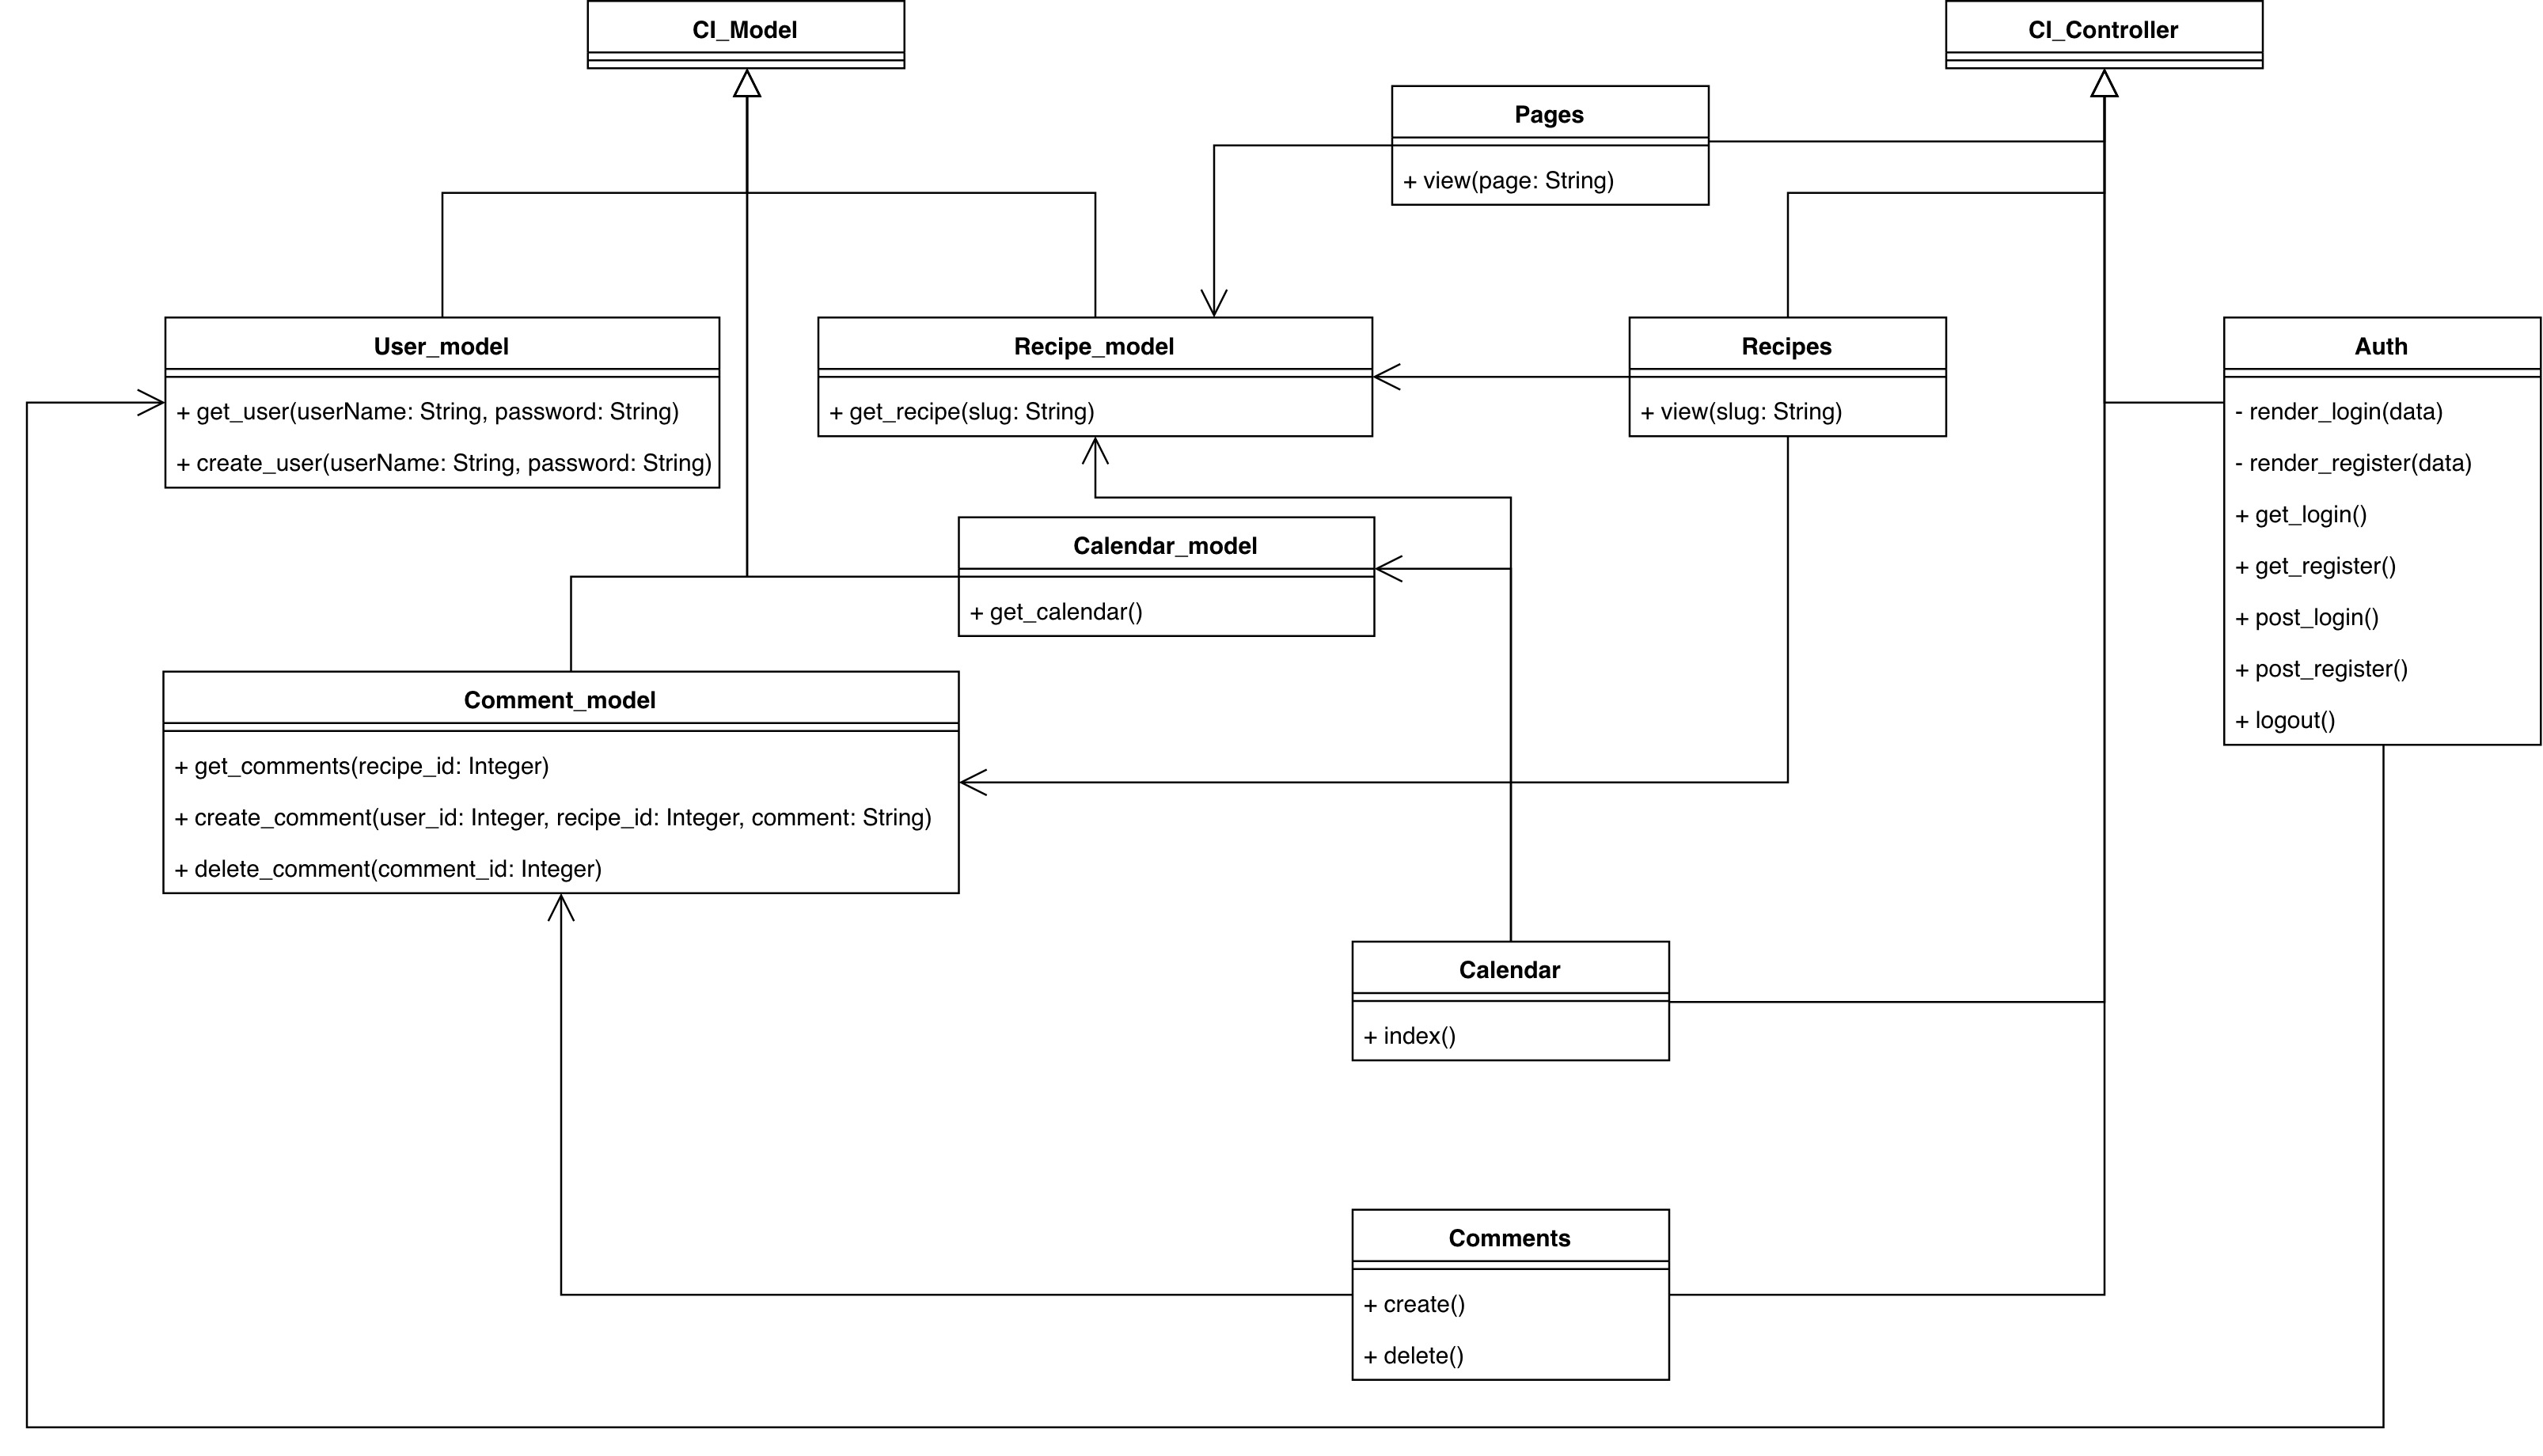
\includegraphics[width=\linewidth]{images/class-diagram.jpg}
		\caption{Class diagram of Receps Recept}
		\label{fig:class-diagram}
	\end{center}
\end{figure}

All the code except for the View code is object-oriented. No code exists outside classes, as well as no static methods. Also all the code is clearly divided according to the MVC pattern. This means:
\begin{itemize}
	\item There is nothing related to HTTP or HTML outside the view.
	\item There is nothing related to databases outside the model layer.
	\item There exists no logic in the model layer.
\end{itemize}

\subsection{Security}
Three security factors where considered when coding the web site. They were \textit{Input Filtering}, \textit{Database security}, and \textit{Password Encryption}.

\subsubsection{Input Filtering}
CodeIgniter provides a validator that can be used to validate form data on the server, preferably before using the data. Figure \ref{fig:auth-login} shows the code that runs when a user logs in. The form validator is used to check that there exists both a username and a password. The validator is then run and if the validator returns false an error will be displayed, as well as the user not getting to log in. Input filtering is also about preventing SQL-injection attacks and CodeIgniter automatically escape strings if you use the built in query builder active record class, which always was used. The next chapter further covers database management in CodeIgniter.

\begin{figure}
\begin{lstlisting}[frame=single, numbers=left, breaklines=true, basicstyle=\ttfamily\footnotesize, firstnumber=60]
public function post_login()
{
  $this->form_validation->set_rules('username', 'Username', 'required');
  $this->form_validation->set_rules('password', 'Password', 'required');

  if ($this->form_validation->run() === false) {
    $data['error'] = true;
    .
    .
    .
\end{lstlisting}
\caption{Part of auth controller (\href{https://github.com/juliuscc/kth-id1354/blob/master/homework-3/application/controllers/Auth.php\#L60}{Auth.php}) that handles login}
\label{fig:auth-login}
\end{figure}

\subsubsection{Database security}
Database security is a broad subject. One obvious aspect is password protecting both the root user on the database but also having an extra user with limited access for the web server to use. This was configured and the limited privileges are shown in figure \ref{fig:database-privileges}. Another very important aspect is protecting against SQL-injection attacks. As previously mentioned CodeIgniter has built in support for escaping data. If active records are used to build queries the data is escaped. Figure \ref{fig:sql-injection} shows code from the comment model where CodeIgniters built in query builder is used to build a query to get all user comments. CodeIgniter also supports prepared statements, called query bindings, however because active records are easier to use and offer the same security, they were used.

\begin{figure}
	\begin{center}
		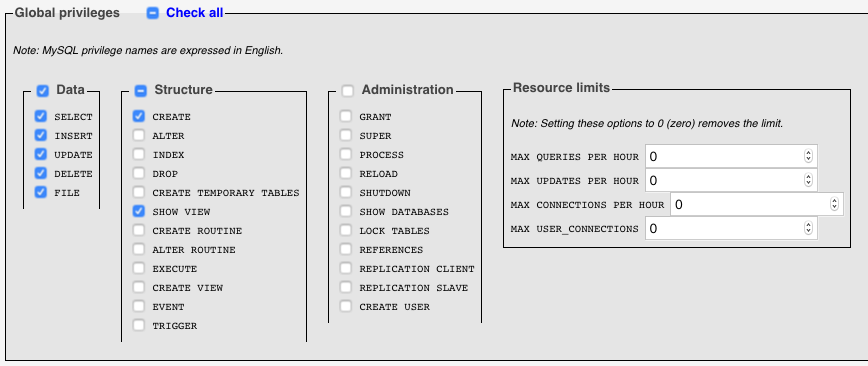
\includegraphics[width=0.7\linewidth]{images/database-privileges.png}
		\caption{Database priviliges for the user receps-recept}
		\label{fig:database-privileges}
	\end{center}
\end{figure}

\begin{figure}
\begin{lstlisting}[frame=single, numbers=left, breaklines=true, basicstyle=\ttfamily\footnotesize, firstnumber=9]
public function get_comments($recipe_id)
{
  $this->db->select('*');
  $this->db->where('recipe_id', $recipe_id);
  $this->db->from('comments');
  $this->db->join('users', 'comments.user_id = users.user_id');

  $query = $this->db->get();

  return $query->result();
}
\end{lstlisting}
\caption{Part of comment model (\href{https://github.com/juliuscc/kth-id1354/blob/master/homework-3/application/models/Comment\_model.php\#L9}{Comment\_model.php}) that handles login}
\label{fig:sql-injection}
\end{figure}

\subsubsection{Password Encryption}
No user passwords were saved in cleartext. The cryptographically safe hash function bcrypt was used. New users passwords were hashed with the PHP-function \textit{password\_hash}. The password for users who wanted to log in were verified with the PHP-function \textit{password\_verify}.

\subsection{Performance}
The performance of a web site is very important, and one of the more critical factors is the usage of caches, as often the largest delay is caused by internet latency. Large front-end files (both CSS and JS) can also cause a long render time, which is why there exists lighter frameworks like Elm and Preact, as alternatives for React, Vue, and Angular. The web server used Apache 2.2.34, which comes with an enabled cache, to reduce database calls and PHP execution. The more important cache is web-cache which is used. Figure \ref{fig:web-cache} shows how web cache is used to greatly improve loading times, where all files except the html-file is cached.

\begin{figure}
	\begin{center}
		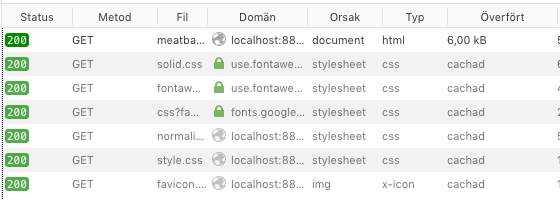
\includegraphics[width=0.7\linewidth]{images/web-cache.png}
		\caption{Screenshot of network statistics when visiting web page}
		\label{fig:web-cache}
	\end{center}
\end{figure}

\subsection{Database}
All data was stored in a MySQL database. It was very easy to work with a database using CodeIgniters built in query builders. Figure \ref{fig:auth-login} shows how complex queries were built.

\section{Discussion}

There were two mandatory and two optional tasks for this assignment. They were:

\begin{enumerate}
	\item \textbf{Mandatory:} MVC Architecture with (or without) a PHP Framework
	\item \textbf{Mandatory:} Security
	\item \textbf{Optional:} Improve Performance
	\item \textbf{Optional:} Use a Database
\end{enumerate}

\noindent
Every requirement was met. It was the first time I have used a PHP framework. I first used Laravel but it was very complicated to get to work. The biggest difference between CodeIgniter and Laravel compared to web frameworks I have used is that the core files are not in any way hidden. Working with Express.js or Next in Node, is a very different experience. There all framework files are imported and hidden, leaving only your code in the project. Of course there exists one folder called \texttt{node\_modules} where all the code exists but you do not open that folder and it is completely hidden. A benefit with Laravel compared to Express is that Laravel handles a lot more. You can basically write your models, configure what database you want to use, and then type \texttt{php artisan migrate} and Laravel handles the creation of tables in the database. This is a big upgrade from having to manually configure database creation.

\section{Comments About the Course}

This is a good course. I did not really like doing the UML-diagram especially when the line is blurry between my code and the frameworks code.

\printbibliography[heading=bibintoc]

\end{document}
